\chapter{\IfLanguageName{dutch}{Stand van zaken}{State of the art}}
\label{ch:stand-van-zaken}

% Tip: Begin elk hoofdstuk met een paragraaf inleiding die beschrijft hoe
% dit hoofdstuk past binnen het geheel van de bachelorproef. Geef in het
% bijzonder aan wat de link is met het vorige en volgende hoofdstuk.

% Pas na deze inleidende paragraaf komt de eerste sectiehoofding.

In de inleiding is duidelijk geworden dat het onderzoek gericht zal zijn op twee mogelijke dataformaten aan de hand van 2 verschillende structuren, namelijk JSON aan de hand van REST en gRPC aan de hand van Protocol Buffers. Om dit onderzoek volledig te kunnen begrijpen is het belangrijk om de werking en de basisprincipes van deze dataformaten en de daarbij behorende structuren te begrijpen. Om deze reden zullen eerst de werking en basisprincipes van JSON en REST worden uitgelegd, en als volgt die van gRPC en Protocol Buffers.

\section{JSON}
\label{sec:JSON}

\subsection{Algemeen}
\label{subsec:Algemeen}

JavaScript Object Notation of in het kort, JSON, is zoals beschreven in Standard ECMA-404 ~\autocite{Json2017} een tekstsyntaxis of dataformaat dat geïnspireerd is door de object literalen van JavaScript dat ook gekend staat als ECMAScript. Het maakt een gegevensuitwisseling tussen alle programmeertalen op een gestructureerde manier mogelijk. Hiervoor maakt JSON gebruik van een structuur van accolades, haakjes, dubbele punten en komma's dewelke zeer nuttig kan zijn in verschillende contexten, profielen en applicaties. Ondanks dat JSON geïnspireerd is door ECMAScript probeert het de interne data representatie ervan niet op te leggen aan andere programmeertalen, in plaats daarvan deelt JSON een onderdeel van ECMAScript's syntax met alle andere programmeertalen. 

JSON mag niet gezien worden als een specificatie van een volledige gegevensuitwisseling want dat is het ook niet. Bij een zinvolle gegevensuitwisseling wordt er een overeenstemming over de semantiek die gekoppeld is aan een gebruik van de JSON-syntaxis tussen producent en consument vereist. JSON kan wel gezien worden als een syntactisch raamwerk waaraan een specifieke semantiek kan worden gekoppeld.

Doordat er veel verschillende types getallen zijn zoals, maar niet beperkt tot, decimale en binaire getallen, kiest JSON voor enkel een weergave van getallen die mensen gebruiken, namelijk een reeks cijfers. Ook al zijn alle programmeertalen het niet altijd eens over de interne representaties van getallen, ze weten wel hoe ze cijferreeksen moeten begrijpen.

Zoals nu wel duidelijk is kunnen programmeertalen sterk verschillen in mate van wat ondersteund wordt en hoe iets moet gerepresenteerd worden. Dit geldt ook voor objecten, niet alle programmeertalen ondersteunen objecten, en indien ze dit wel doen is er nog steeds een groot verschil in de kenmerken en beperkingen de objecten bieden. Met andere woorden kunnen de modellen van objectsystemen heel erg uiteenlopen. Om dit probleem aan te pakken biedt JSON een eenvoudige notatie aan voor het uitdrukken van verzamelingen met naam / waarde-paren. Om zulke verzamelingen weer te geven hebben de meeste programmeertalen reeds een functie zoals maar niet beperkt tot, struct, map, hash, object.
Daarnaast biedt JSON ook ondersteuning voor geordende zoeklijsten, alsook hiervoor hebben alle programmeertalen een functie om deze weer te geven zoals array, vector en list. Aangezien objecten en arrays zich kunnen nesten kunnen aan de hand van JSON complexe structuren zoals boomstructuren worden gerepresenteerd.

Hieruit kan dus geconcludeerd worden dat door het aanvaarden van JSON's simpele conventies, complexe datastructuren uitgewisseld kunnen worden tussen wat anders incompatibele programmeertalen zijn.



\subsection{Achterliggend}
\label{subsec:Achterliggend}

Een JSON-tekst bestaat uit een reeks tokens die gevormd zijn uit Unicode-codepunten en die in overeenstemming zijn met de JSON-waardegrammatica. Deze reeks tokens bevat tekenreeksen, cijfers, zes structurele token en drie letterlijke naamtokens.
Hieronder volgt een opsomming van de zes structurele tokens en de drie literal name tokens samen met de bijhorende Unicode.

De zes structurele tokens:

\begin{itemize}
    \item $\rbrack$ Linker vierkante haak, U+005B
    \item $\rbrack$ Rechter vierkante haak, U+005D
    \item \{ Linker accolade, U+007B
    \item \} Rechter accolade, U+007D
    \item : Dubbele punt, U+003A
    \item , Komma, U+002C
\end{itemize}

De drie literal name tokens:

\begin{itemize}
    \item true      U+0074 U+0072 U+0075 U+0065
    \item false     U+0066 U+0061 U+006C U+0073 U+0065
    \item null      U+006E U+0075 U+006C U+006C 
\end{itemize}

Voor of na een token is het toegestaan om onbelangrijke witruimte te gebruiken. Witruimte kan beschreven worden als een willekeurige reeks van één of meerdere van onderstaande codepunten.

\begin{itemize}
    \item Tekentabel        U+0009
    \item Regelinvoer       U+000A
    \item Regelterugloop    U+000D
    \item Spatie            U+0020
\end{itemize}

Witruimte is niet in elke token toegestaan, een spatie is hierop een uitzondering en is wel toegestaan in strings.

\subsection{Waarden}
\label{subsec:Waarden}

De bovengestelde tokens vormen de ruggengraad van een JSON-bestand, echter is het de bedoeling dat een JSON-bestaand iets van data overdraagd. Deze data kan aan de hand verschillende waarden worden voorgesteld, namelijk als objecten, arrays, nummers, strings, true, false, null.

\begin{figure}[h]
    \centering
    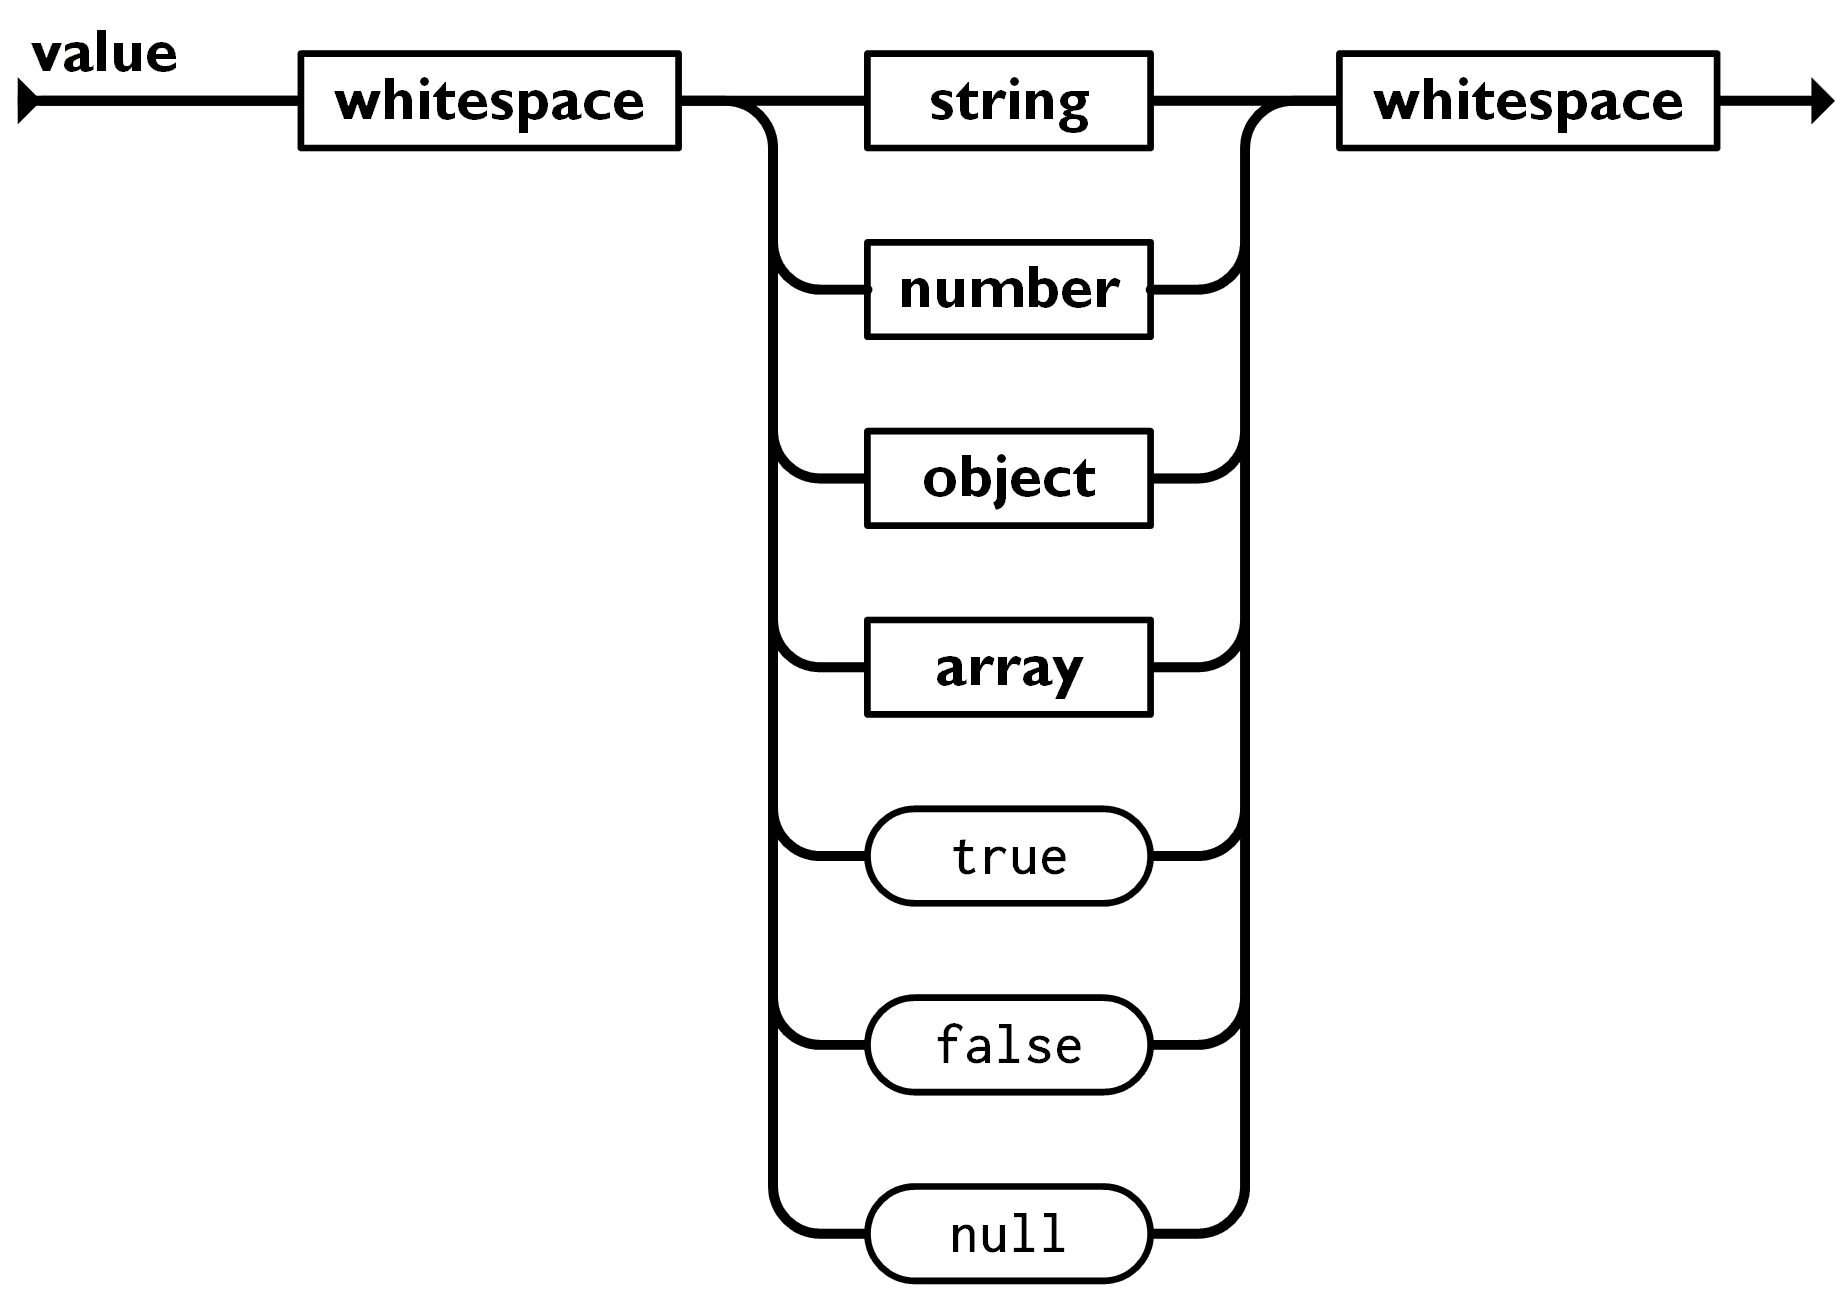
\includegraphics[scale=0.75]{jsonValue}
   \caption[JSON values]{De structuur van een JSON-waarde met alle mogelijke waarden die deze kan bevatten}
   \label{fig:jsonValue}
\end{figure}

De eerste waarden die besproken worden zijn de objecten, deze worden voorgesteld over een paar accolades die geen of meerdere name/value paren kunnen incapsuleren zoals te zien is in figuur \ref{fig:jsonObject}. In zo een name/value paar is de naam een string en wordt gevolgd door een dubbele punt die de naam en waarde van elkaar onderscheidt. Optioneel is een komma na de waarde, die de waarde en de eventuele volgende naam van elkaar onderscheiden. De JSON syntax legt geen beperkingen op op vlak van de strings gebruikt als namen. Deze moeten met andere woorden niet uniek zijn en ze moeten geen bepaalde ordening volgen.

\begin{figure}[h]
    \centering
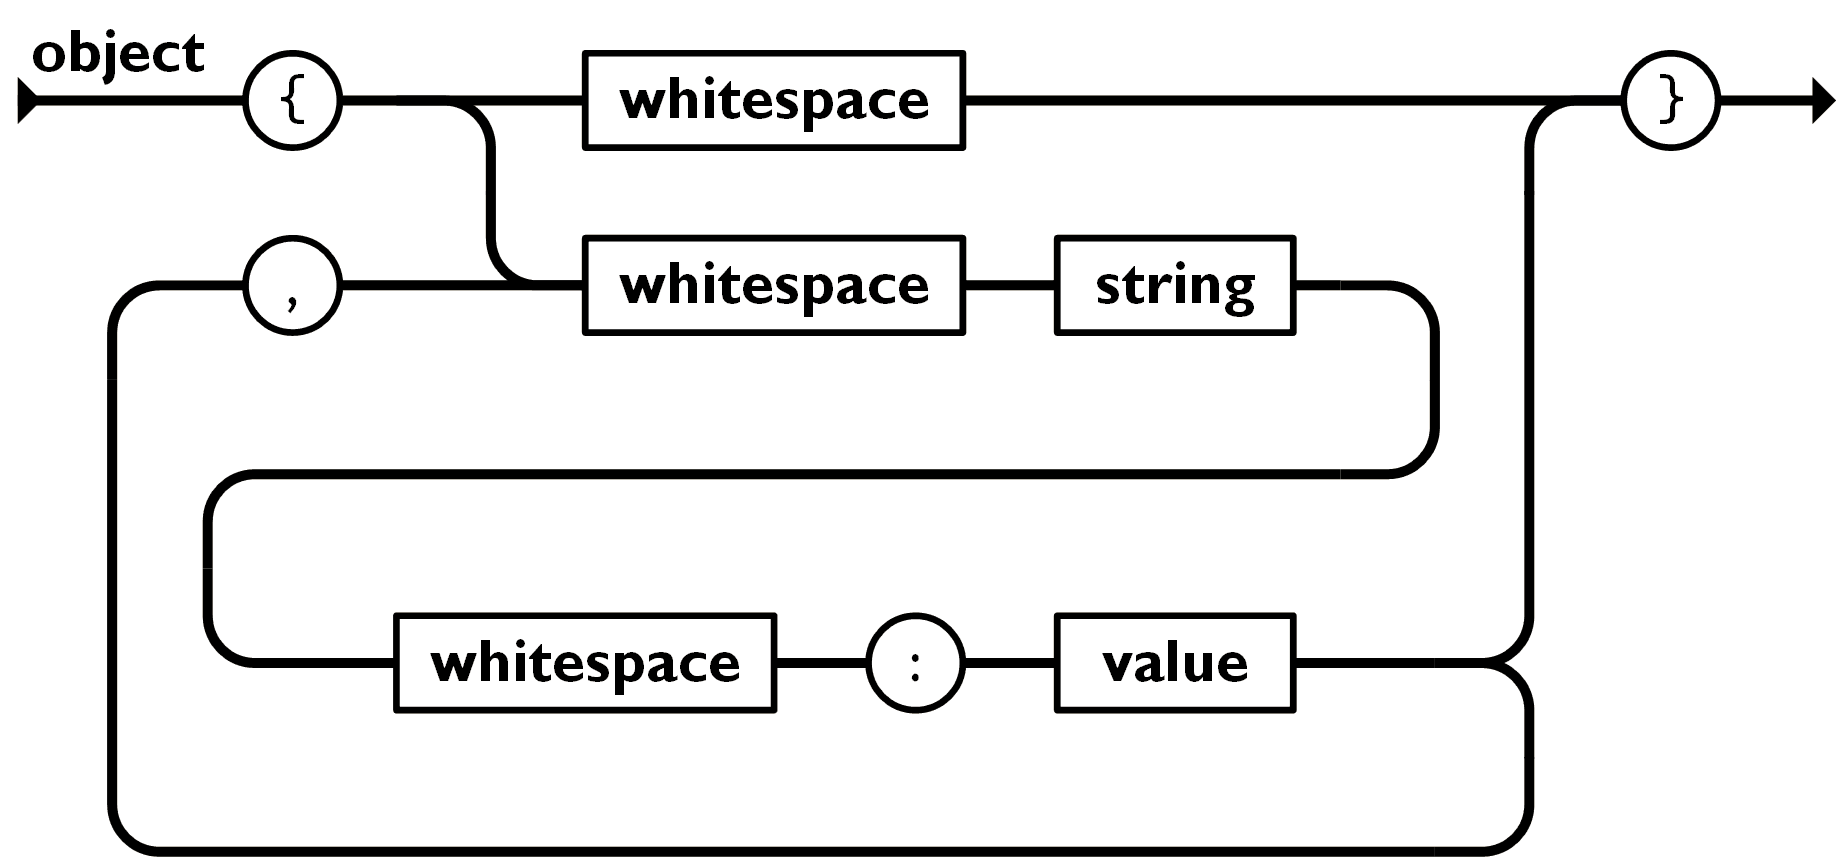
\includegraphics[scale=0.75]{jsonObject}
\caption[JSON Object]{De structuur van een JSON object.}
    \label{fig:jsonObject}
\end{figure}

Een tweede waarde zijn de arrays, dit zijn vierkante haken die geen of meerdere waarden incapsuleren. Het bijzondere aan arrays is dat deze niet beperkt zijn tot een name/value paar maar dat deze zelf dus meerdere waarden en dus ook andere arrays kunnen bevatten en dus genest kunnen worden. Dit kan afgeleid worden uit figuur \ref{fig:jsonArray}. De array structuur wordt net zoals bij objecten geen beperkingen opgelegd op vlak van de ordening van de waarden, echter wordt de array structuur vooral gebruikt in situaties waar de ordening wel enig belang heeft.

\begin{figure}[h]
    \centering
    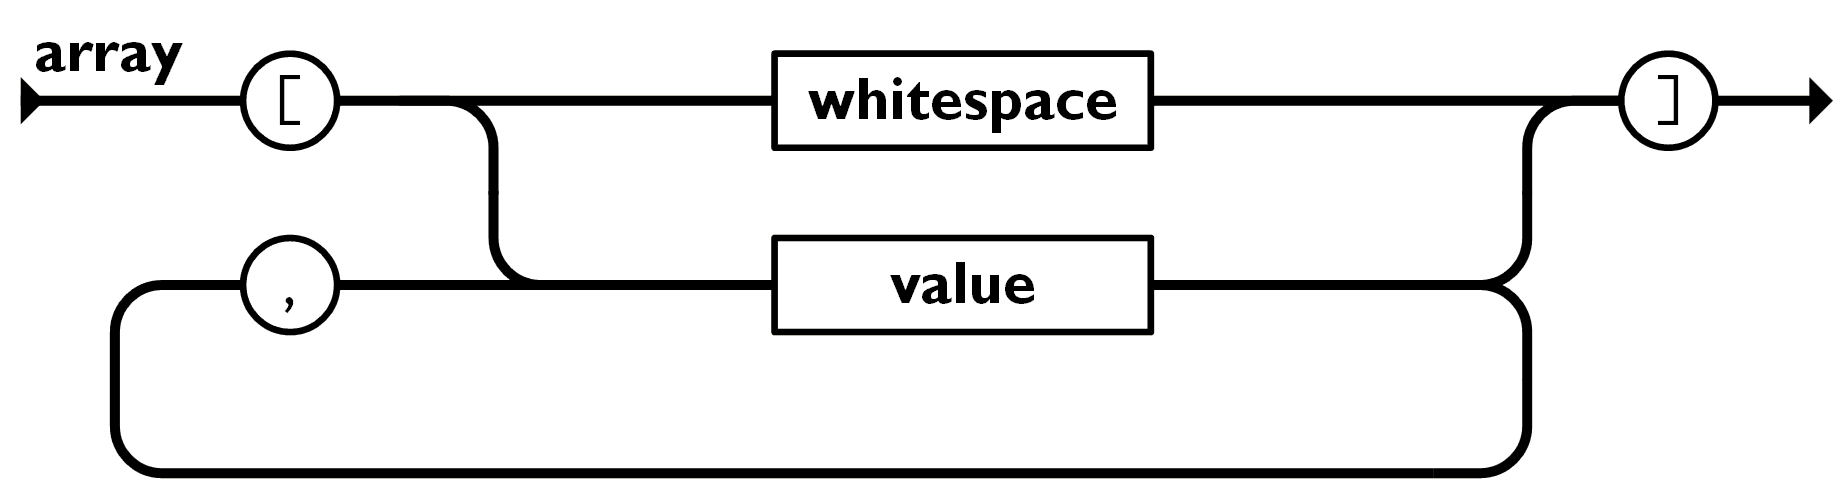
\includegraphics[scale=0.75]{jsonArray}
    \caption[JSON Array]{De structuur van een JSON array.}
    \label{fig:jsonArray}
\end{figure}






